\chapter{Sprint 3}
\label{chap:sprint3}
The following section presents an overview of how we planned, worked and
completed sprint.

Sprint 3 started on 1st of October and ended on 14th of October, giving it a duration of 14 days. 
% The length of the sprints were discussed with the customer and the advisor, and all agreed on 14 days as a suitable length of a sprint.\\

The chapter is divided into five parts, starting with the overall plan for the
sprint in Section \ref{sec:sprint3sprintplan}. Followed by the sprint backlog, which
enlists the tasks that have been chosen for the sprint. Section
\ref{sec:sprint3designAndImplementation}.
will focus on the work made to the GUI, the logic implemented in the application and the work done to the database and database access in the applications.
The chapter ends with what have been tested and the corresponding results in
Section \ref{sec:sprint3testingAndResults} and a sprint review in Section
\ref{sec:sprint3sprintRetrospective}.

\section{Sprint Plan}
\label{sec:sprint3sprintplan}
The plan for the sprint was to work on the distraction, the log, the reminders and the database connection. 
We also planned to do some work on the report, due to an expected preliminary delivery.

Regarding the distraction, the plan was to make some kind of distraction through the Karotz.

Regarding the log, the plan was to work on a better solution of the calendar view and make the backend 
connections for saving the log in the database.

Regarding the reminders the plan was to finish the work on inplementing the reminders and making the reminder 
work through the Karotz.

Regarding the database the plan was to make different SQL-query methods for medications, reminders, 
instructions and similiar.

\section{Sprint backlog}
This section contains a table with the sprint backlog, which is a smaller part of the product backlog. The 
goal is to implement the entire sprint backlog during the sprint.

\begin{table}
	\begin{center}
		\begin{tabular}{|p{2.0cm}| p{8.0cm}| p{2.0cm}|p{2.0cm}|p{2.0cm}|}
			\hline
			\#  ID 	& Task 	& Story points 	& Estimated hours & Responsible \\
			\hline
			1.1 & Make some kind of distraction through the Karotz & 2 & 10 & Yngve\\
			\hline
			1.2 & Make method for saving a treatment through Karotz & 4 & 20 & Yngve \\
			\hline
			1.3 & Make method for starting treatment through Karotz & 2 & 10 & Yngve \\
			\hline
			2.1 & Calendar view for log & 3 & 15 & Esben \\
			\hline
			2.2 & Backend solution for saving elements to the log & 9 & 45 & Esben\\
			\hline
			3.1 & Make the reminder for Android devices & 4 & 20 & Eirik\\
			\hline
			3.2 & Make the reminder for Karotz & 5 & 25 & Yngve\\
			\hline
			3.3 & User interface for changing reminder preferences & 6 & 30 & Eirik and Aleksander\\
			\hline
			3.4 & Secure that the reminder is giving independently of internet connection and sound level on the phone & 2 & 10 & Eirik\\
			\hline
			4.1 & Make SQL-queries for LogModel & 1 & 5 & Esben \\
			\hline
			4.2 & Make SQL-queries for essential database fields for CAPP, including avatar, shop, rewards and so on & 3 & 15 & \\
			\hline
			4.3 & Make SQL-queries for Medications & 2 & 10 & Esben and J\o rgen \\
			\hline
			4.4 & Make SQL-queries for Notifications & 2 & 10 & J\o rgen \\
			\hline
			4.5 & Make SQL-queries for Instructions & 1 & 5 & J\o rgen \\
			\hline
			4.6 & Make the SQL-queries updater for Karotz & 3 & 15 & Yngve \\
			\hline
			4.7 & Make a generic JSON-deserializer  & 1 & 5 & Yngve and Esben \\
			\hline
			4.8 & Make JSON-deserializer for logmodel & 1 & 5 & Esben\\
			\hline
			4.9 & Make JSON-deserializer for instructions & 1 & 5 & Esben\\
			\hline
			\bfseries{SUM} & & \bfseries{52} & \bfseries{260} & \\
			\hline
			\hline
		\end{tabular}
	\end{center}
	\caption{Backlog for sprint 3}
\end{table}

\section{Design and Implementation}
\label{sec:sprint3designAndImplementation}
We continued to add graphical user interface elements to represent the different functionality 
in the applications. During the sprint the focus has been on the log, the reminders, the Karotz and the database. 
The reason for this was the priorities given by the customer.  

\subsection{User Interface Layer}
During the sprint we made GUI-changes to the log and the instructions. The instructions will now 
show a list of the different medicines. When a medicine is selected, a new screen with a picture 
and instructions for correct use is shown. This is downloaded from an external server, which makes 
it easier to change the pictures without updating the applications. 


During the sprint the reminders were implemented. When the reminder is set off by the logic layer, 
the screen will show a message with the text ``It's time to take your medicine''. 

During the sprint we, in cooperation with the customer started to work on making better screen 
elements like buttons, images and similar in order to replace all text. Since CAPP 
will be used by young children, it will be more understandable for children if we use pictures, rather than text. This process was 
started so late in the sprint that the results are to be expected during the next sprint. 

\subsection{Application Logic Layer}
The reminders have been added, as mentioned previously. At this point, the alarm will be set off by 
pressing a button inside the application. An alarm manager calculates an offset of ten seconds and 
then fires an alarm. When the user clicks on the alarm sign, he/she is taken to the treatment screen. 
The functionality for choosing custom alarm times is yet to be implemented.

\subsection{Data Persistence Layer}
More web access modules have been added, and some of the previous modules have been altered. The new pages include:
\begin{itemize}
  \item \emph{dose\_is\_taken.php:} Check if a dose of a planned medicine has been taken that day.
  \item \emph{get\_instructions.php:} Get instructions (image, effect description and usage description) for a given medicine by ID.
  \item \emph{get\_log\_for\_child.php:} Returns all registered entries for the day for a given child (id) during the given month during the given year.
\end{itemize}
I addition to the new modules, \emph{get\_doses\_for\_current\_state.php} has been altered to only return doses for the day that has not been taken already.

\subsection{Karotz}
This subsection has not been present in the other sprint reports. Because the Karotz is a 
separate part of the system from the Android applications and the database, we felt
it was important to add a it as a separate section.

The Karotz will now play reminders at a specific time set by the user in the database. The
reminder starts a distraction process, which makes the Karotz able to act as a distraction 
during treatment. It will play sound in order to tell the user which medicine to take, 
how to take them and then count down from 10 to 0 to work as a distraction. There are some 
problems with the calibration of sound messages and the countdown, so the Karotz may skip 
messages, making it sound like it skips numbers when counting.

The applications communicate with the Karotz through the database by saving and retrieving 
data asynchronously and without direct messages between them.

\section{Testing and Results}
\label{sec:sprint3testingAndResults}

\subsection{Testing}
During this sprint we tested the reminder and the log part of the system. We wanted
to make sure that the reminder was given regardless of phone state, such as when the phone is asleep, or if the the phone
is used in a call. 

We had had some problems coloring the correct days, and making the log the way we wanted, so we felt we had to make
sure it was done correctly, and working in the way we wanted. We therefore did testing focusing on the log.

Testing the Karotz is essential to the project, so in this sprint the two most important modules of the Karotz app
were tested: notification and medication. There was also an additional test to check whether several medications
happening at the same time would be handled correctly.

There was a problem with the treatment functionality of the Karotz. The countdown did not work correctly. Often jumping from ten to seven, from seven to three and from three to finished. This is because the Karotz' built-in media player is slow and takes a little
time to start and stop. The solution to this problem is to include the entire countdown in one audio file, compared to
previously where each number was stored in a seperate file.

\begin{table}
	\begin{center}
		\begin{tabular}{|p{3.0cm}|p{14.0cm}|}
			\hline
			\bf{Item} & \bf{Description}\\
			\hline
			\bf{ID} & UNIT3.1\\
			\bf{Description} & Test that the alarm is given independently of phone state\\
			\bf{Date} & 14.10.2012\\
			\bf{Responsible} & Eirik\\
			\bf{Subject} & AlarmReciever and MainMenu (which sets the alarm)\\
			\bf{Precondition} & Working version of CAPP, runable on the android virtual device\\
			\bf{Steps} &
			\begin{tabulenum}
				\item Press the ``notify us'' button to set the alarm.
				\item Wait until the alarm activates.
				\item Observe if the alarm activates if you are on a call.
				\item Observe if the alarm activates if you're in another application.
				\item Observe if the alarm activates if the phone have been switched off.
			\end{tabulenum}\\
			\hline
			\bf{Results} & The alarm worked fine, unless if the phone is switched off, which releases all alarms. We found a solution to this
			by adding an \code{onBootAction}.\\
			\hline
		\end{tabular}
	\end{center}
	\caption{Unit test 3.1: Alarm when turned off}
	\label{tab:unit3.1}
\end{table}

\begin{table}
	\begin{center}
		\begin{tabular}{|p{3.0cm}|p{14.0cm}|}
			\hline
			\bf{Item} & \bf{Description}\\
			\hline
			\bf{ID} & UNIT3.2\\
			\bf{Description} & Test that the correct days is colored in the log \\
			\bf{Date} & 09.10.2012\\
			\bf{Responsible} & Esben\\
			\bf{Subject} & \code{LogModelParser}, \code{CalendarView}\\
			\bf{Precondition} & Correct resultset from \code{get\_log\_for\_child.php}\\
			\bf{Steps} & \begin{tabulenum}
			  \item Press ``log''.
			  \item Compare the colored days with the resultset from \code{get\_log\_for\_child.php}.
			\end{tabulenum}\\
			\hline
			\bf{Results} & 
				Correct days was ultimatly colored after a huge effort was made in finding a couple of bugs.\\
			\hline
		\end{tabular}
	\end{center}
	\caption{Unit test 3.2: Calendar colors}
	\label{tab:unit3.2}
\end{table}

\begin{table}
	\begin{center}
		\begin{tabular}{|p{3.0cm}|p{14.0cm}|}
			\hline
			\bf{Item} & \bf{Description}\\
			\hline
			\bf{ID} & UNIT3.3\\
			\bf{Description} & Test that a notification is given at the correct time through the Karotz\\
			\bf{Date} & 09.10.2012\\
			\bf{Responsible} & Yngve\\
			\bf{Subject} & Karotz app's \code{Repository} and \code{Notification} modules\\
			\bf{Precondition} & Karotz app starts, planned dose URLs and parameters are correct\\
			\bf{Steps} &
			\begin{tabulenum}
				\item Adjust a time for the notification in the table \code{MEDICAL\_PLAN\_DOSES} in the database.
				\item Wait until the alarm activates.
				\item Observe if the notification is activated at the correct time.
			\end{tabulenum}\\
			\hline
			\bf{Results} & The notification went off at the given time. \\
			\hline
		\end{tabular}
	\end{center}
	\caption{Unit test 3.3: Karotz Notification}
	\label{tab:unit3.3}
\end{table}

\begin{table}
	\begin{center}
		\begin{tabular}{|p{3.0cm}|p{14.0cm}|}
			\hline
			\bf{Item} & \bf{Description}\\
			\hline
			\bf{ID} & UNIT3.4\\
			\bf{Description} & Test that a distraction is started and works correctly when the button on the Karotz is pressed after a notification is given. \\
			\bf{Date} & 09.10.2012\\
			\bf{Responsible} & Yngve\\
			\bf{Subject} & Karotz app's \code{Repository}, \code{Notification} and \code{Medication} modules\\
			\bf{Precondition} & Notification is given correctly throug the karotz \\
			\bf{Steps} &
			\begin{tabulenum}
				\item Wait until the notification activates.
				\item Press the button to terminate the notification and start medication.
				\item Follow the vocal instructions given by the Karotz.
				\item Observe that the medication procedure is starting.
				\item Observe that the countdown works correctly.
				\item Observe that a reward (credits) is given at the end of the medication process.
				\item Observe that the reward is saved in the database. 
			\end{tabulenum}\\
			\hline
			\bf{Results} & The medication process started, but the countdown started but skipped some numbers. This can however be solved by
			making the whole countdown in a single sound file. The Karotz expressed audiably that a reward was given, and that was saved to
			the database. \\
			\hline
		\end{tabular}
	\end{center}
	\caption{Unit test 3.4: Karotz distraction}
	\label{tab:unit3.4}
\end{table}

\begin{table}
	\begin{center}
		\begin{tabular}{|p{3.0cm}|p{14.0cm}|}
			\hline
			\bf{Item} & \bf{Description}\\
			\hline
			\bf{ID} & UNIT3.5\\
			\bf{Description} & Test that several doses in the same notification will make a medication for each dose, after each other.\\
			\bf{Date} & 11.10.2012\\
			\bf{Responsible} & Yngve\\
			\bf{Subject} & Karotz app's \code{Repository}, \code{Notification} and \code{Medication} modules\\
			\bf{Precondition} & A notification that consists of three doses is given. \\
			\bf{Steps} &
			\begin{tabulenum}
				\item Wait for a notification with three doses at the same time.
				\item Observe that the first medication process is completed correctly.
				\item Observe that when the first medication process is done, another is started automatically.
				\item Observe that the second medication process is completed correctly.
				\item Observe that when the second medication process is done, another is started automatically.
				\item Observe that the third medication process is completed correctly.
				\item Observe that when the third medication process is done, no other process is started and the Karotz returns to idle state.
			\end{tabulenum}\\
			\hline
			\bf{Results} & The medication series worked as expected. \\
			\hline
		\end{tabular}
	\end{center}
	\caption{Unit test 3.5: Several doses in a medication}
	\label{tab:unit3.5}
\end{table}

In addition to these tests, we are testing the application continuously.
\subsection{Results}
We found out that the alarm was given regardless of the phone state, unless the phone was turned off, since we have
no way to turn the phone back on. The alarms will be put back on whenever the phone is turned on, so the only scenario
the alarm will not be given is if the phone is turned off at the time for a reminder.
Regarding the coloring of the days in the log, the color depends on the medication plan followed that day. We had some trouble
discovering what bugs made the wrong days be colored, but after extensive debugging, we found out that one of the SQL-querys was not correct. Upon fixing the query to gather the right ID from the database the log worked as intended.

\section{Sprint Retrospective}
\label{sec:sprint3sprintRetrospective}
This section contains an evaluation of the Sprint. The evaluation is done mainly by us, but feedback from the customers is added to the retrospect.

\subsection*{What went well?}
Karotz is ready for user testing. 
Eirik was responsible for Aleksanders' tasks when he was gone, and secured progress.
Communication with the customer has improved.

\subsection*{What shall we start doing?}
We identified one element that we should add to our sprints:
\begin{enumerate}
	\item Increase amount of programming sessions. %TODO: EXPLAIN
\end{enumerate}

\subsection*{What could have gone better?}
We forgot to have daily standups, this shouldn't happen.
Better testing of the Karotz in advance to the customer meeting.
Be better prepared in advance of customer meeting.


\subsection*{What should we stop doing?}
We felt that nothing was done completely wrong during this sprint.

\subsection{Sprint Burndown Chart}

\begin{figure}
	\begin{center}
		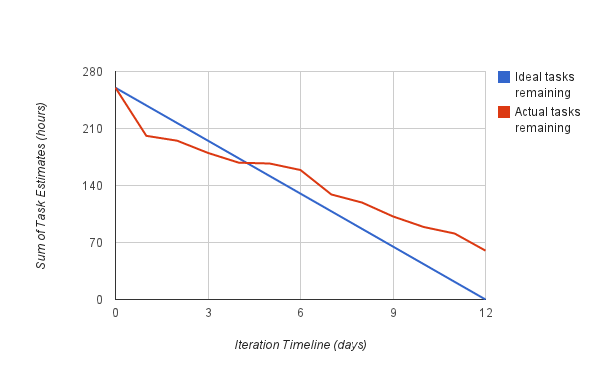
\includegraphics[width=15cm]{Pictures/Charts/Sprint3burndown}
	\end{center}
	\caption{Sprint 3 burndown chart}
	\label{fig:sprint3burndown}
\end{figure}

\begin{table}
	\centering
	\begin{sideways}
		\begin{tabular}{| l | p{6.5cm} | c | c | c | c |l |}
			\hline
			  \#  ID 	& Task 	& Story points 	& Estimated & Actual &
			  Estimated Left & Responsible \\
			\hline
			  1.1 & Make some kind of distraction through Karotz & 2 & 10 & 3 & 0 & Yngve\\
			\hline
			  1.2 & Make method for saving a treatment through Karotz & 4 & 20 & 8 & 0 & Yngve\\
			\hline
			  1.3 & Make method for starting treatment through Karotz & 2 & 10 & 5 & 0 & Yngve\\
			\hline
			  2.1 & Calendar view for log & 3 & 15 & 15 & 3 & Esben\\
			\hline
			  2.2 & Backend solution for saving the log & 9 & 45 & 5 & 25 & Esben\\
			\hline
			3.1 & Make the reminder for Android Platform & 4 & 20 & 20 & 2 & Eirik \\
			\hline
			3.2 & Make the reminder for Karotz & 5 & 25 & 25 & 0 & Yngve\\
			\hline
			3.3 & User interface for changing reminder preferences & 6 & 30 & 4 & 28 & Aleksander and Eirik\\
			\hline
			3.4 & Secure that the reminder is giving independently of internet connection and sound level on the phone & 2 & 10 & 10 & 2 & Eirik\\
			\hline
			4.1 & Make SQL-queries for LogModel & 1 & 5 & 4 & 0 & Esben \\
			\hline
			4.2 & Make SQL-queries for essential database fields for children application, including avatar, shop, rewards and so on & \sout{3} & \sout{15} & Task dropped & Task dropped & -- \\
			\hline
			4.3 & Make SQL-queries for Medications & 2 & 10 & 7 & 0 & Esben and J\o rgen\\
			\hline
			4.4 & Make SQL-queries for Notifications & 2 & 10 & 0 & 0 & J\o rgen\\
			\hline
			4.5 & Make SQL-queries for Instructions & 1 & 5 & 3 & 0 & J\o rgen\\
			\hline
			4.6 & Make the SQL-queries updater for Karotz & 3 & 15 & 3 & 0 & Yngve\\
			\hline
			4.7 & Make a generic JSON-deserializer & 1 & 5 & 10 & 0 & Yngve and Esben\\
			\hline
			4.8 & Make JSON-deserializer for logmodel & 1 & 5 & 5 & 0 & Esben\\
			\hline
			4.9 & Make JSON-deserializer for instructions & 1 & 5 & 5 & 0 & Esben\\
			\hline
			\bfseries{SUM} & & \bfseries{49} & \bfseries{245} & \bfseries{114} & \bfseries{60} & \\
			\hline
			\hline
		\end{tabular}
	\end{sideways}
	\caption{Sprint Retrospective, Sprint 3}
	\label{tab:sprint3burndown}
\end{table}
Figure \ref{fig:sprint3burndown} and table \ref{tab:sprint3burndown} show the sprint 
burndown chart for sprint 3. The burndown chart looks good at first glance, compared to sprint 1 and 2. During the last two sprints we have learned more about estimation and development, this has resulted in a steadier pace. The burndown charts started out very good, this was due to some functionality being dropped very early in the sprint. This decision was made by 
the customer.

Also we discovered fairly early that some tasks were easier than expected. Closer to the end 
of week one the burndown chart flattened out a bit. The reason behind this is that we 
needed to work intensly on assignments in other courses. At the start of week two, a programming 
session was held, resulting in a steep decline in the burndown chart. After this the pace was 
fairly consistent.

We had a goal of finishing 49 story points. There are 60 hours left, which with the 
multiplier we used, 5, means there are $60/5=12$ story poinst left. Ergo, we finished
$49-12=37$ story points, which is closer to the ideal projected effort than the previous sprints, 
but not satisfactory.
\clearpage{}
\blankpage{}